% Define the top matter
\setModuleTitle{ChIP-Seq}
\setModuleAuthors{%
  Remco Loos, EMBL-EBI \mailto{remco@ebi.ac.uk} \\
  Myrto Kostadima \mailto{kostadim@ebi.ac.uk} \\
  Sonika Tyagi \mailto{sonika.tyagi@agrf.org.au}
}
\setModuleContributions{%
  Xi Li \mailto{sean.li@csiro.au}%
}

%  Start: Module Title Page
\chapter{\moduleTitle}
\newpage
% End: Module Title Page

\section{Key Learning Outcomes}

After completing this practical the trainee should be able to:
\begin{itemize}
  \item Perform simple ChIP-Seq analysis, e.g. the detection of immuno-enriched areas using the chosen peak caller program MACS
  \item Visualize the peak regions through a genome browser, e.g. Ensembl, and identify the real peak regions
  \item Perform functional annotation and detect potential binding sites (motif) in the predicted binding regions using motif discovery tool, e.g. MEME.
\end{itemize}

\section{Resources You'll be Using}
 
\subsection{Tools Used}
\begin{description}[style=multiline,labelindent=0cm,align=left,leftmargin=0.5cm]
  \item[MACS]\hfill\\
  	\url{http://liulab.dfci.harvard.edu/MACS/index.html}
  \item[Ensembl]\hfill\\
  	\url{http://www.ensembl.org}
  \item[PeakAnalyzer]\hfill\\
  	\url{http://www.ebi.ac.uk/bertone/software}
  \item[MEME]\hfill\\
  	\url{http://meme.ebi.edu.au/meme/tools/meme}
  \item[TOMTOM]\hfill\\
  	\url{http://meme.ebi.edu.au/meme/tools/tomtom}  
  \item[DAVID]\hfill\\
  	\url{http://david.abcc.ncifcrf.gov}
  \item[GOstat]\hfill\\
    \url{http://gostat.wehi.edu.au}
\end{description}

\subsection{Sources of Data}
  \url{http://www.ebi.ac.uk/arrayexpress/experiments/E-GEOD-11431}
 % These data are reported in Chen, X et al. (2008) Integration of external signaling pathways with the core tran-scriptional network in embryonic stem cells. Cell. Jun 13;133(6):1106-17.


\newpage

\section{Introduction}

\begin{information}
The goal of this hands-on session is to perform some basic tasks in the analysis
of ChIP-seq data. In fact, you already performed the first step, alignment of
the reads to the genome, in the previous session. We start from the aligned
reads and we will find immuno-enriched areas using the peak caller MACS. We will
visualize the identified regions in a genome browser and perform functional
annotation and motif analysis on the predicted binding regions.
\end{information}

\section{Prepare the Environment}

\begin{information}
The material for this practical can be found in the \texttt{ChIP-seq} directory on your
desktop. This directory also contains an electronic version of this document,
which can be useful to copy and paste commands. Please make sure that this
directory also contains the SAM/BAM files you produced during the alignment
practical.
\end{information}

\begin{steps}
If you didn't have time to align the control file called \texttt{gfp.fastq}
during the alignment practical, please do it now. Follow the same steps, from
the bowtie2 alignment step, as for the \texttt{Oct4.fastq} file.
\end{steps}

%\begin{note}
%In ChIP-seq analysis (unlike in other applications such as RNA-seq) it can be useful
%to exclude all reads that map to more than one location in the
%genome. When using Bowtie2, this can be done using the
%\texttt{-m 1} option, which tells it to report only unique matches (See
%\texttt{bowtie2 --help} for more details).
%\end{note}

\begin{steps}
Open the Terminal and go to the \texttt{chipseq} directory:
\begin{lstlisting}
cd ~/chipseq
\end{lstlisting}
\end{steps}

\section{Finding enriched areas using MACS}

\begin{information}
MACS stands for Model based analysis of ChIP-seq. It was designed for
identifying transcription factor binding sites. MACS captures the influence of
genome complexity to evaluate the significance of enriched ChIP regions, and
improves the spatial resolution of binding sites through combining the
information of both sequencing tag position and orientation. MACS can be easily
used for ChIP-Seq data alone, or with a control sample to increase specificity.
\end{information}

\begin{steps}
Consult the MACS help file to see the options and parameters:

\begin{lstlisting}
macs --help
\end{lstlisting}
\end{steps}

\begin{information}
The input for MACS can be in ELAND, BED, SAM, BAM or BOWTIE formats (you just
have to set the \texttt{--format} option).

Options that you will have to use include: 

\begin{description}[style=multiline,labelindent=0cm,align=right,leftmargin=\descriptionlabelspace,rightmargin=1.5cm,font=\ttfamily]
 \item[-t] To indicate the input ChIP file.
 \item[-c] To indicate the name of the control file.
 \item[--format] To change the file format. The default format is bed.
 \item[--name] To set the name of the output files.
 \item[--gsize] This is the mappable genome size. With the read length we have,
 $70\%$ of the genome is a fair estimation. Since in this analysis we include
 only reads from chromosome 1 (197Mbases), we will use a \texttt{--gsize} of 138Mbases (70\% of 197Mbases).
 \item[--tsize] To set the read length (look at the FASTQ files to check the
 length).
 \item[--wig] To generate signal wig files for viewing in a genome browser.
 Since this process is time consuming, it is recommended to run MACS first with
 this flag off, and once you decide on the values of the parameters, run MACS
 again with this flag on.
 \item[--diag] To generate a saturation table, which gives an indication whether
 the sequenced reads give a reliable representation of the possible peaks.
\end{description}
\end{information}

\begin{steps}
Now run macs using the following command:

\begin{lstlisting}[style=command_syntax]
macs -t <Oct4_aligned_bam_file> -c <gfp_aligned_bam_file> --format=BAM --name=Oct4 --gsize=138000000 --tsize=26 --diag --wig 
\end{lstlisting}

Look at the output saturation table (\texttt{Oct4\_diag.xls}). To open this file
file, right-click on it and choose ``Open with'' and select LibreOffice. Do you think
that more sequencing is necessary?

Open the Excel peak file and view the peak details. Note that the number of tags
(column 6) refers to the number of reads in the whole peak region and not the
peak height.

\end{steps}

\section{Viewing results with the Ensembl genome browser}

\begin{information}
It is often instructive to look at your data in a genome browser. Before, we
used IGV, a stand-alone browser, which has the advantage of being installed
locally and providing fast access. Web-based genome browsers, like Ensembl or
the UCSC browser, are slower, but provide more functionality. They do not only
allow for more polished and flexible visualisation, but also provide easy access
to a wealth of annotations and external data sources. This makes it
straightforward to relate your data with information about repeat regions, known
genes, epigenetic features or areas of cross-species conservation, to name just
a few. As such, they are useful tools for exploratory analysis.

They will allow you to get a `feel' for the data, as well as detecting
abnormalities and problems. Also, exploring the data in such a way may give you
ideas for further analyses.
\end{information}

\begin{steps}
Launch a web browser and go to the Ensembl website at
\url{http://www.ensembl.org/index.html}

Choose the genome of interest (in this case, mouse) on the left side of the
page, browse to any location in the genome or click one of the demo links
provided on the web page.

%\includegraphics[width=\trainerIconWidth]{../photos/MoustHome.pdf}

\begin{figure}[H]
\centering
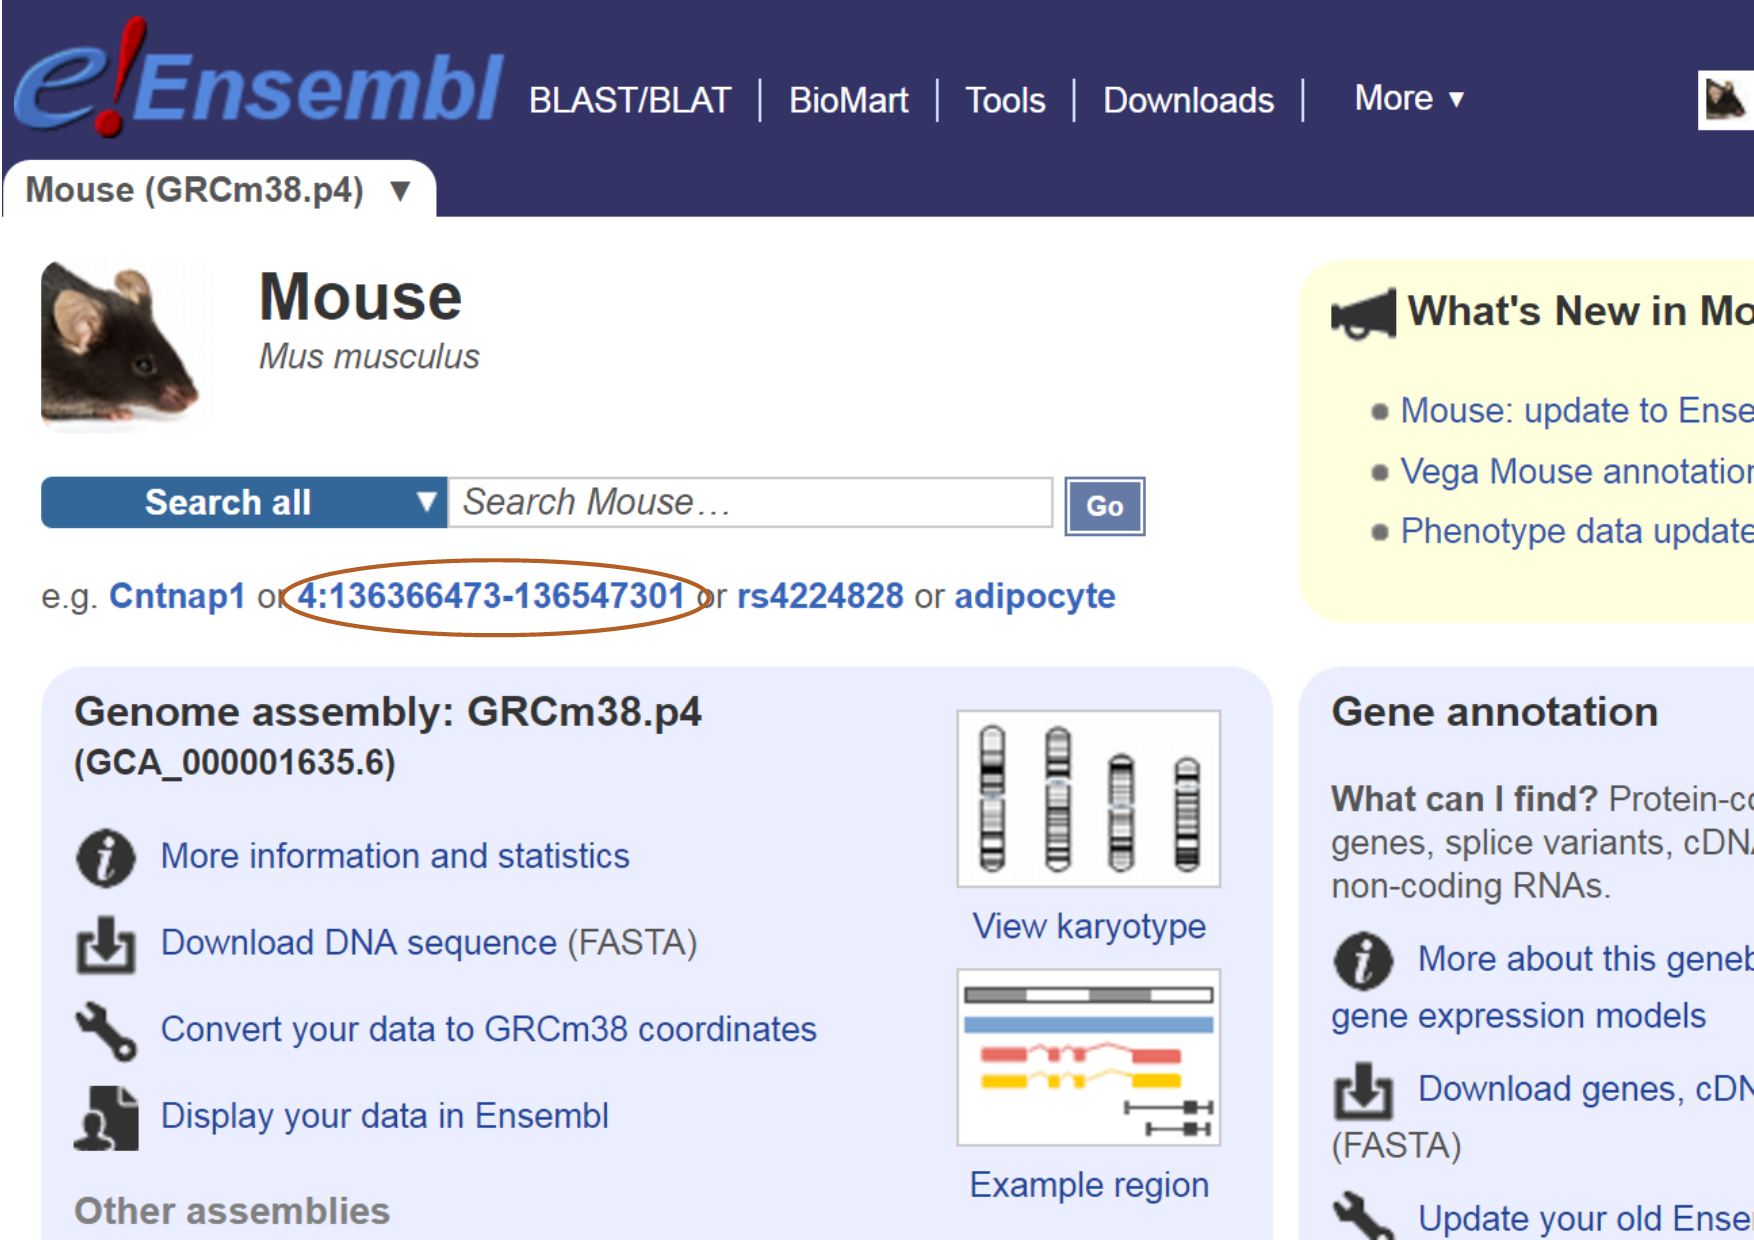
\includegraphics[width=0.8\textwidth]{MouseHome.png}
\caption{Ensembl Mouse Homepage}
\label{fig:MouseHome}
\end{figure}



Click on the \textbf{Add your data} link on the left, then choose
\textbf{Add your data} in the \textbf{Custom Data} tab.

\begin{figure}[H]
\centering
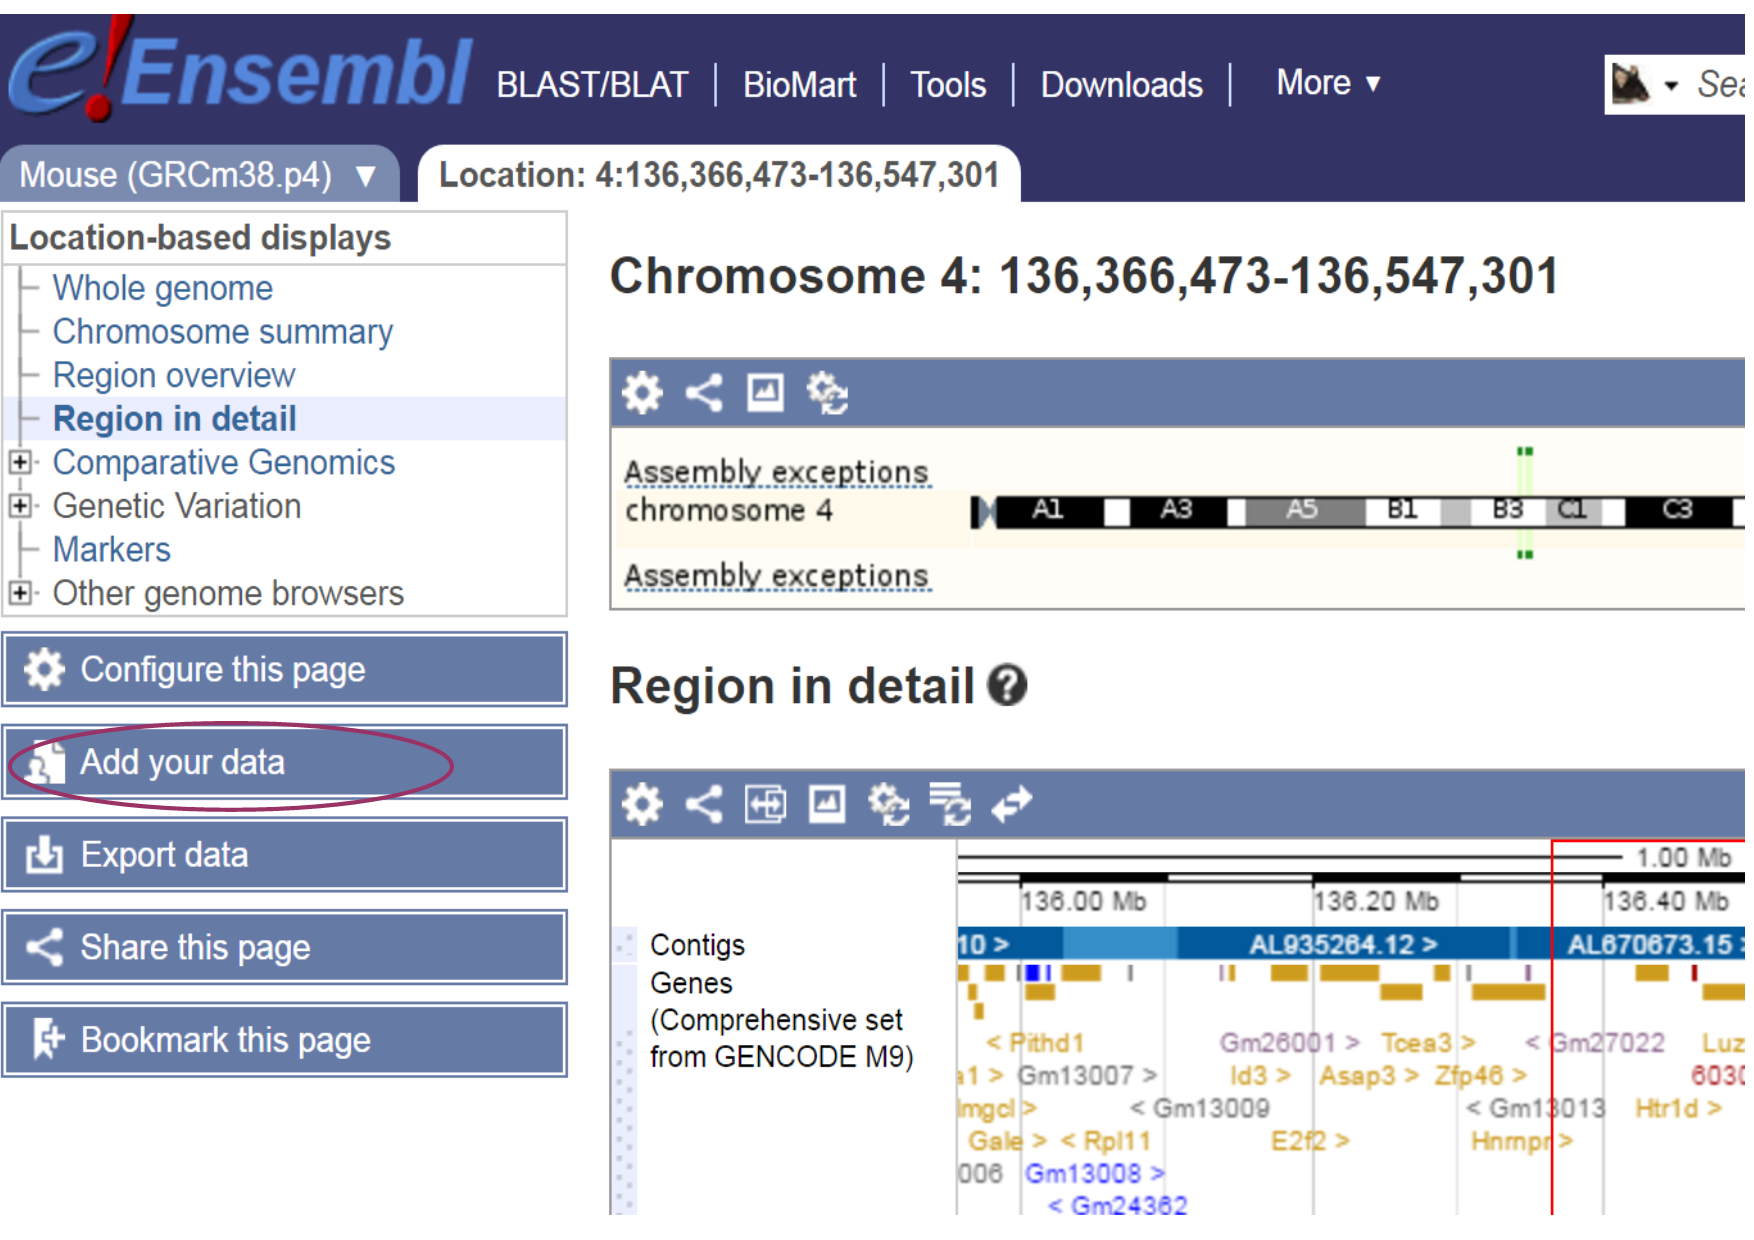
\includegraphics[width=0.8\textwidth]{AddData.png}
\caption{Click Add your data link}
\label{fig:AddData}
\end{figure}

\end{steps}

\begin{note}
Wig files are large so are inconvenient for uploading directly to the Ensemble Genome browser. Instead, we will convert it to an indexed binary format
and put this into a web accessible place such as on a HTTP, HTTPS, or FTP server.
This makes all the browsing process much faster. Detailed
instructions for generating a bigWig from a wig type file can be found at:

\url{http://genome.ucsc.edu/goldenPath/help/bigWig.html}.

\end{note}

\begin{steps}
We have generated bigWig files in advance for you to upload to the Ensembl
browser. They are at the following URL:
\url{http://www.ebi.ac.uk/~remco/ChIP-Seq_course/Oct4.bw} (Please right click and choose ``Copy Link Address'' to copy the URL).

To visualise the data:
\begin{itemize}
	\item Paste the location above in the Data field. 
	\item Set data format bigWig. 
	\item Choose some informative name
        \item Click Add data and in the next window choose the colour of your preference. 
	\item Click \textbf{Save} and close the window to return to the genome browser. 
\end{itemize}

\begin{figure}[H]
\centering
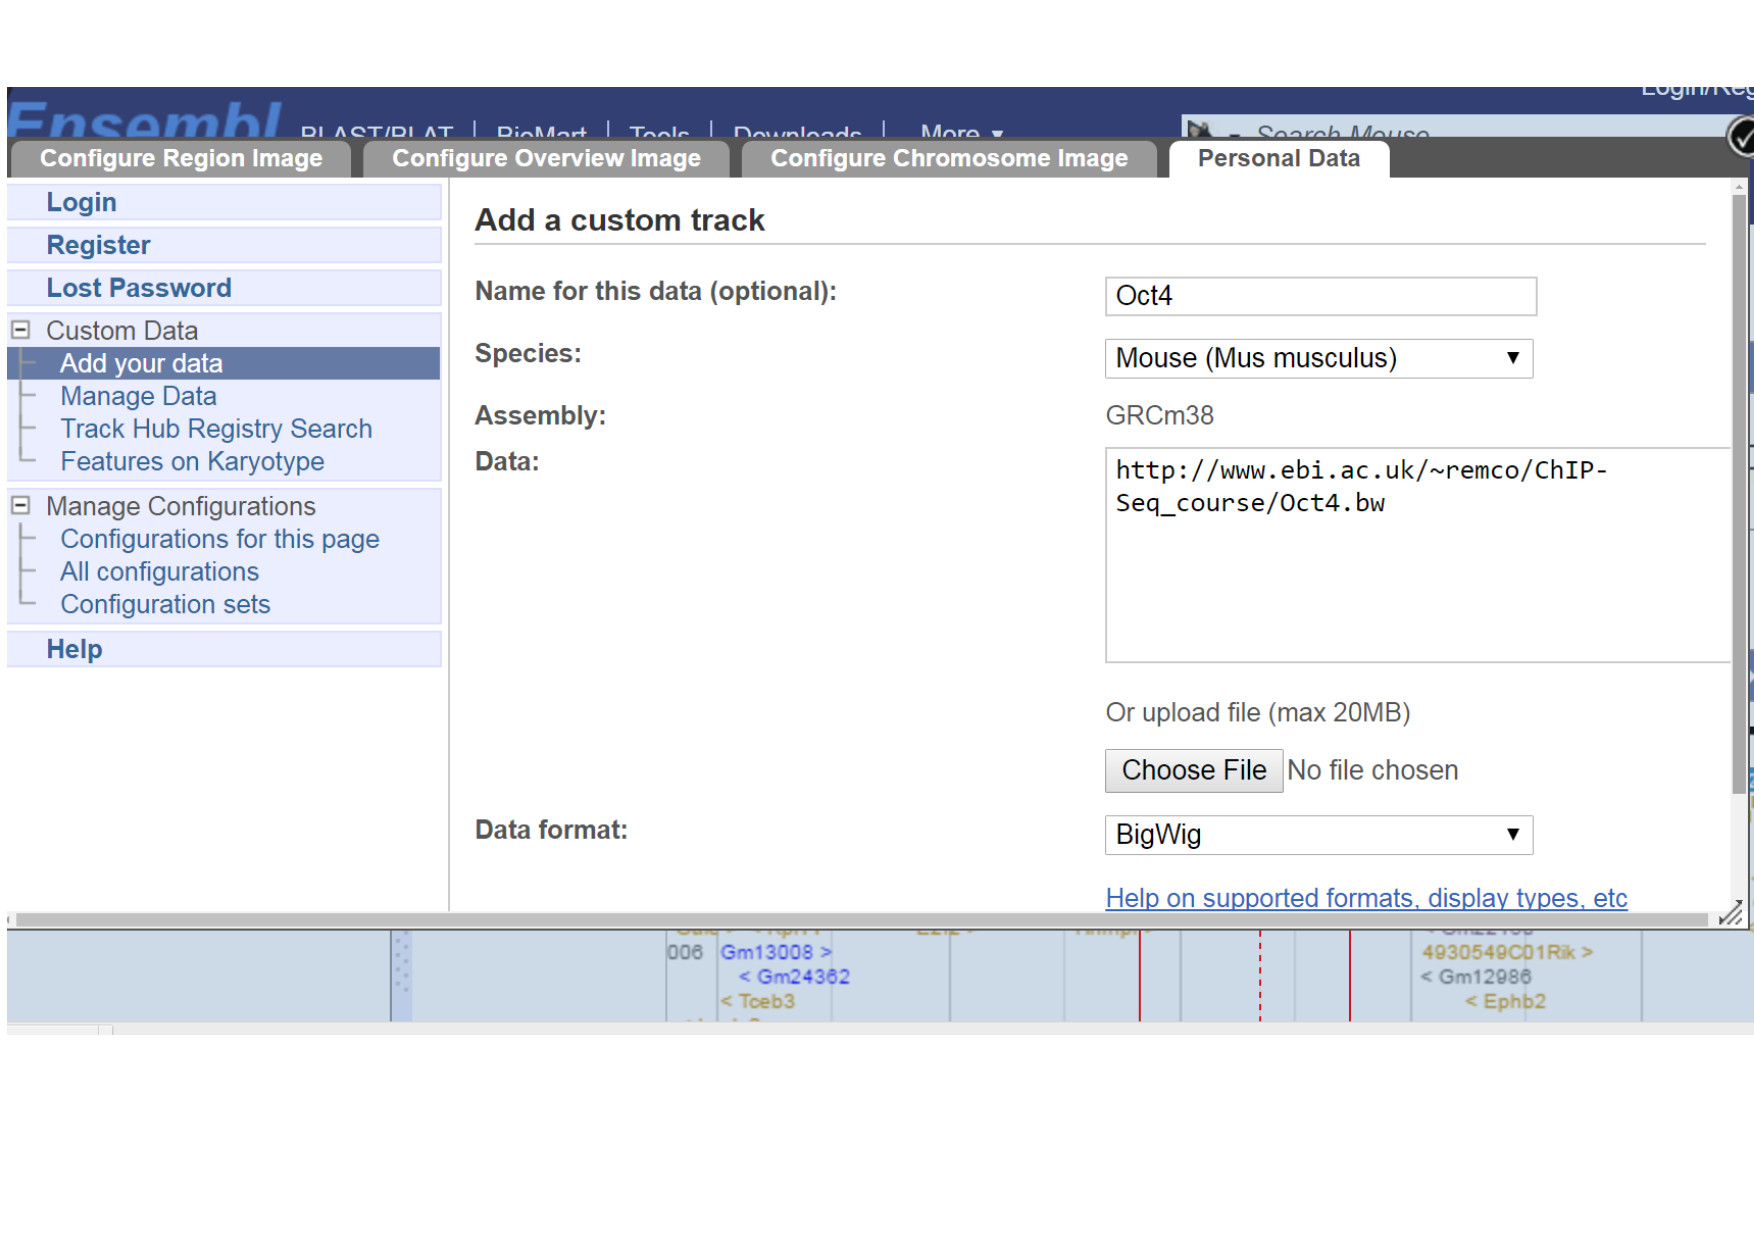
\includegraphics[width=0.8\textwidth]{UploadURL.png}
\caption{Upload the bigWig file to Ensembl}
\label{fig:UploadURL}
\end{figure}

Repeat the process for the gfp control sample, located at:

\url{http://www.ebi.ac.uk/~remco/ChIP-Seq_course/gfp.bw} (Please right click and choose ``Copy Link Address'' to copy the URL).

After uploading, to make sure your data is visible:
\begin{itemize}
        \item Switch to the \textbf{Configure Region Image} tab
        \item Click \textbf{Your data} in the left panel
        \item Choose each of the uploaded *.bw files to confirm the \textbf{Wiggle plot} in \textbf{Change track style} pop up menu has been choosen.
        \item Closing the window will save these changes.

\end{itemize}

\begin{figure}[H]
\centering
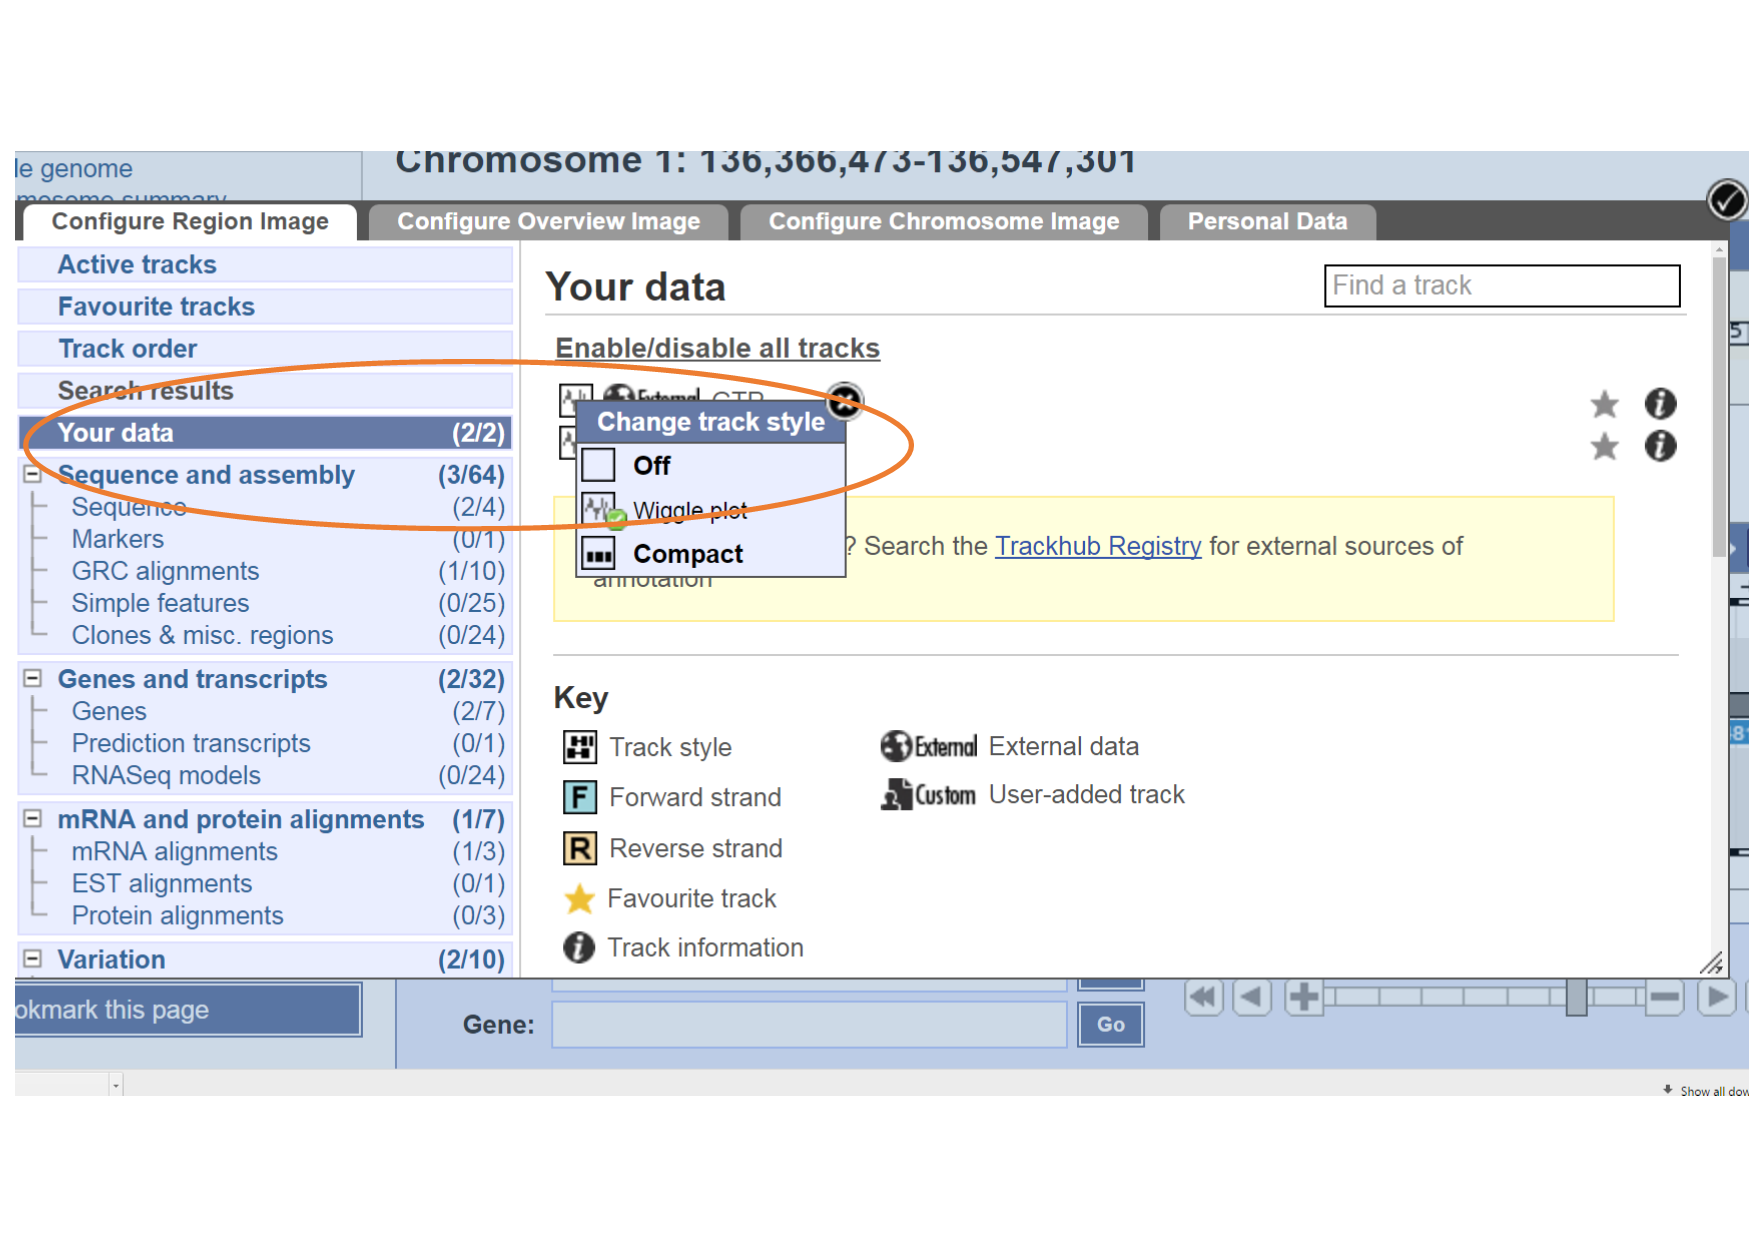
\includegraphics[width=0.8\textwidth]{ConfigureYourData.png}
\caption{Make sure your uploaded data are visible in the browser}
\label{fig:ConfigureYourData}
\end{figure}

Go to a region on chromosome 1 (e.g. \texttt{1:34823162-35323161}), and zoom in and out
to view the signal and peak regions. Be aware that the y-axis of each track is auto-scaled independently of each other,
so bigger-looking peaks may not actually be bigger! Always look at the values
on the left hand side axis.
\end{steps}

\begin{questions}
What can you say about the profile of Oct4 peaks in this region? 
\begin{answer}
There are no significant Oct4 peaks over the selected region.
\end{answer}

Compare it with H3K4me3 histone modification wig file we have generated at 
\url{http://www.ebi.ac.uk/~remco/ChIP-Seq_course/H3K4me3.bw} . 
\begin{answer}
H3K4me3 has a region that contains relatively high peaks than Oct4. 
\end{answer}

Jump to \texttt{1:36066594-36079728} for a sample peak. Do you think H3K4me3
peaks regions contain one or more modification sites? What about Oct4?
\begin{answer}
Yes. There are roughly three peaks, which indicate the possibility of having more than one modification sites in this region. 

For Oct4, no peak can be observed.
\end{answer}

\end{questions}

\begin{note}
MACS generates its peak files in a file format called bed file. This is a simple
text format containing genomic locations, specified by chromosome, begin and end
positions, and some more optional information.

See \url{http://genome.ucsc.edu/FAQ/FAQformat.html#format1} for details.

Bed files can also be uploaded to the Ensembl browser.
\end{note}

\begin{advanced}
Try uploading the peak file generated by MACS to Ensembl. Find the first peak and the peak with the highest score (the fifth column) in
the file and see if the peak looks convincing to you.
\end{advanced}


\section{Annotation: From peaks to biological interpretation}

\begin{information}
In order to biologically interpret the results of ChIP-seq experiments, it is
usually recommended to look at the genes and other annotated elements that are
located in proximity to the identified enriched regions. This can be easily done
using PeakAnalyzer.
\end{information}

\begin{steps}
Go to the PeakAnalyzer tool directory:
\begin{lstlisting}
cd ~/chipseq/peakanalyzer/1.4
\end{lstlisting}
Launch the PeakAnalyzer program by typing:
\begin{lstlisting}
java -jar PeakAnalyzer.jar &
\end{lstlisting}

The first window allows you to choose between the split application (which we
will try next) and peak annotation. Choose the peak annotation option and click
\textbf{Next}.

We would like to find the closest downstream genes to each peak, and the genes
that overlap with the peak region. For that purpose you should choose the
\textbf{NDG} option and click \textbf{Next}.

Fill in the location of the peak file \texttt{Oct4\_peaks.bed}, and choose the mouse GTF
as the annotation file. You don't have to define a symbol file since gene
symbols are included in the GTF file.

Choose the output directory and run the program.
\end{steps}

\begin{information}
When the program has finished running, you will have the option to generate
plots, by pressing the \textbf{Generate plots} button. This is only possible if R is
installed on your computer, as it is on this system. A PDF file with the plots will be generated in
the output folder. You could generate similar plots with Excel using the output files that
were generated by PeakAnalyzer. 
\end{information}

\begin{note}
This list of closest downstream genes (contained in the file
\texttt{Oct4\_peaks.ndg.bed}) can be the basis of further analysis. For instance,
you could look at the Gene Ontology terms associated with these genes to get an
idea of the biological processes that may be affected. Web-based tools like
DAVID (\url{http://david.abcc.ncifcrf.gov}) or GOstat
(\url{http://gostat.wehi.edu.au}) take a list of genes and return the enriched
GO categories.
\end{note}

\begin{bonus}
We can pull out Ensemble Transcript IDs from the \texttt{Oct4\_peaks.ndg.bed}
file and write them to another file ready for use with DAVID or GOstat:
\begin{lstlisting}
cut -f 5 Oct4_peaks.ndg.bed | sed '1 d' > Oct4_peaks.ndg.tid
\end{lstlisting}
\end{bonus}

\section{Motif analysis}

\begin{information}
It is often interesting to find out whether we can associate identified the
binding sites with a sequence pattern or motif. We will use MEME for motif
analysis. The input for MEME should be a file in FASTA format containing the
sequences of interest. In our case, these are the sequences of the identified
peaks that probably contain Oct4 binding sites.

Since many peak-finding tools merge overlapping areas of enrichment, the
resulting peaks tend to be much wider than the actual binding sites.
Sub-dividing the enriched areas by accurately partitioning enriched loci into a
finer-resolution set of individual binding sites, and fetching sequences from
the summit region where binding motifs are most likely to appear enhances the
quality of the motif analysis. Sub-peak summit sequences can be retrieved
directly from the Ensembl database using PeakAnalyzer.
\end{information}

\begin{steps}
If you have closed the PeakAnalyzer running window, open it again. If it is
still open, just go back to the first window.

Choose the split peaks utility and click \textbf{Next}. The input consists of
files generated by most peak-finding tools: a file containing the chromosome,
start and end locations of the enriched regions, and a \texttt{.wig} signal file
describing the size and shape of each peak. Fill in the location of both files
\texttt{Oct4\_peaks.bed} and the wig file generated by MACS, which is under the
\texttt{Oct4\_MACS\_wiggle/treat/} directory, check the option to \textbf{Fetch subpeak
sequences} and click \textbf{Next}.

In the next window you have to set some parameters for splitting the peaks.

\begin{description}[style=multiline,labelindent=0cm,align=right,leftmargin=\descriptionlabelspace,rightmargin=1.5cm,font=\ttfamily]
 \item[Separation float] Keep the default value. This value determines when a
 peak will be separated into sub-peaks. This is the ratio between a valley and
 its neighbouring summit (the lower summit of the two). For example, if you set
 this height to be \texttt{0.5}, two sub-peaks will be separated only if the
 height of the lower summit is twice the height of the valley.
 \item[Minimum height] Set this to be \texttt{5}. Only sub-peaks with at least this
 number of tags in their summit region will be separated. Change the organism
 name from the default human to mouse and run the program.
 \item[Organism] Choose \texttt{Mus\_musculus} from the drop down list.
\end{description}
\end{steps}

\begin{information}
Since the program has to read large wig files, it will take a few minutes to
run. Once the run is finished, two output files will be produced. The first
describes the location of the sub-peaks, and the second is a FASTA file
containing 300 sequences of length 61 bases, taken from the summit regions of
the highest sub-peaks.
\end{information}

\begin{steps}
Open a web bowser and go to the MEME website at
\url{http://meme.ebi.edu.au/meme/tools/meme}, and fill in the necessary
details, such as:
\begin{itemize}
	\item Your e-mail address 
	\item The sub-peaks FASTA file \texttt{Oct4\_peaks.bestSubPeaks.fa} (will need uploading), or just paste in the sequences 
	\item The number of motifs we expect to find (1 per sequence) 
	\item The maximum number of motifs to find (3 by default). For Oct4 one classical motif is known 
	\item Click the \texttt{Advanced options}, the width of the desired motif (between 6 to 20)
\end{itemize}
\end{steps}

\begin{note}
You will receive the results by e-mail. This usually doesn't take more than a few minutes.
\end{note}

\begin{steps}
Open the e-mail and click on the link that leads to the HTML results page.

Scroll down until you see the first motif logo. We would like to know if this
motif is similar to any other known motif. We will use TOMTOM for this. Click the right arrow under \texttt{Submit/Download}, and you will see the option \textbf{Tomtom} chosen by default. Click the Submit
button to compare to known motifs in motif databases, and on the new page choose
to compare your motif to those in the ``JASPAR Vertebrates and UniPROBE Mouse''database.
\end{steps}


\begin{questions}
Which motif was found to be the most similar to your motif?
\begin{answer}
Sox2
\end{answer}
\end{questions}

\newpage
\section{Reference}
%TODO Use BibTeX
Chen, X et al.: Integration of external signaling pathways with the core transcriptional network in embryonic stem cells. Cell 133:6, 1106-17 (2008).
